
\section{Circle trigonometry} 

\subsection*{Riding a Ferris Wheel}
Taini is waiting in line to ride the Ferris Wheel.  The bottom of the wheel is 6 feet high so that riders can get in the gondola (seats) and the spokes of the wheel are 47 feet long, which means at the center of the wheel is $47+6=53$ feet high.  A rider in the gondola is always 3 feet below the wheel.

\begin{figure}[htbp]
    \centering
    \scalebox{0.85}{
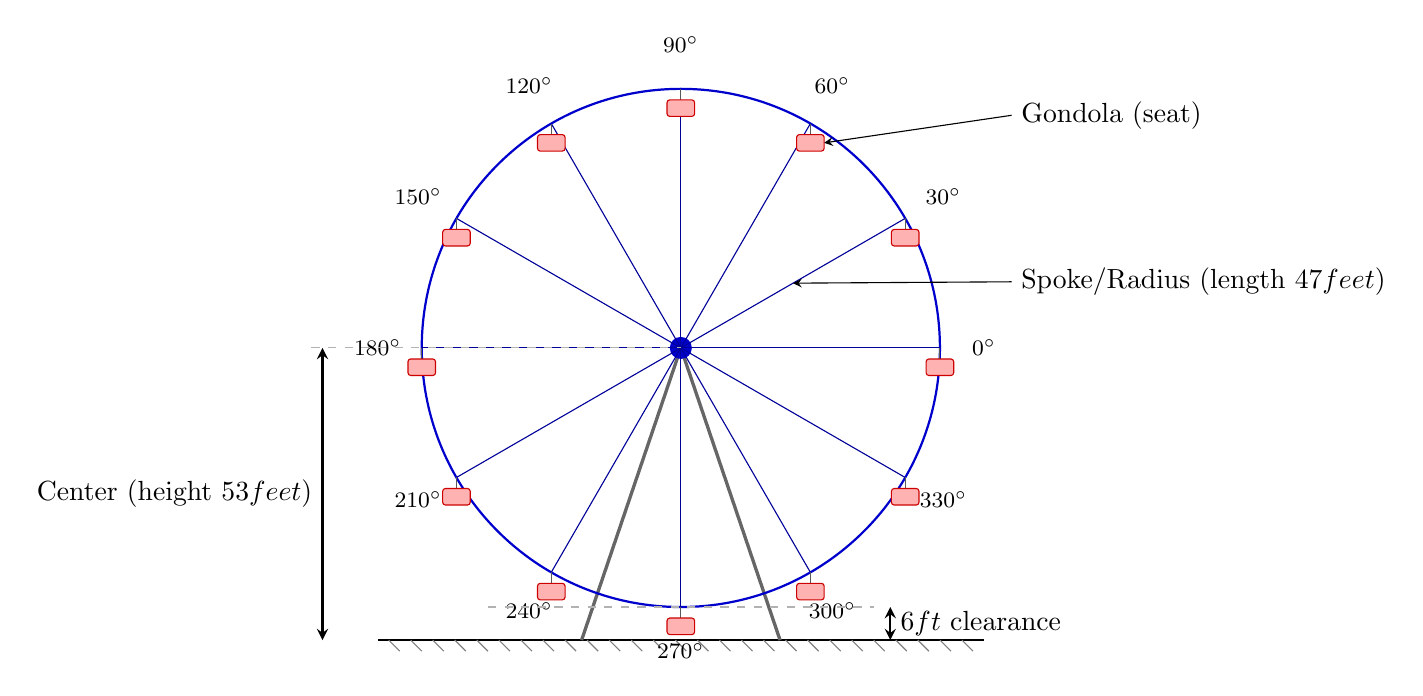
\begin{tikzpicture}[>=stealth, scale=0.07]
  % Define key Y-coordinates (heights)
  \def\groundY{0}
  \def\bottomY{6}
  \def\centerY{53}
  \def\topY{100}
  \def\radius{47}
  \def\centerX{0}
  % Draw Ground (extended further left/right to (-55, 55))
  \draw[thick] (-55, \groundY) -- (55, \groundY);
  \foreach \x in {-53, -49, ..., 53} {
    \draw[gray] (\x, \groundY) -- (\x + 2, \groundY - 2);
  }
  % Draw Center Stand / Support Legs
  \draw[very thick, gray!80!black] (-18, \groundY) -- (\centerX, \centerY) -- (18, \groundY);
  % Draw Outer Wheel and Hub
  \draw[thick, blue!80!black] (\centerX, \centerY) circle (\radius);
  \draw[thick, blue!80!black] (\centerX, \centerY) circle (1.5);
  \fill[blue!80!black] (\centerX, \centerY) circle (2);
  % Draw Spokes (at 30-degree intervals)
  \foreach \angle in {0, 30, ..., 330} {
    \draw[thin, blue!60!black] (\centerX, \centerY) -- ({ \centerX + \radius*cos(\angle) }, { \centerY + \radius*sin(\angle) });
  }
  % Draw Gondolas (Seats) hanging from the rim and angle labels outside
  \foreach \angle in {0, 30, ..., 330} {
    \pgfmathsetmacro{\gx}{\centerX + \radius*cos(\angle)}
    \pgfmathsetmacro{\gy}{\centerY + \radius*sin(\angle)}
    % Gondola hanger
    \draw[gray!70!black] (\gx, \gy) -- (\gx, \gy - 2);
    % Gondola body
    \draw[fill=red!30, draw=red!80!black, rounded corners=1pt] (\gx - 2.5, \gy - 5) rectangle (\gx + 2.5, \gy - 2);
    % Angle Label placed further out (at radius + 8 to clear gondolas)
    \node[font=\footnotesize] at ({ \centerX + (\radius + 8)*cos(\angle) }, { \centerY + (\radius + 8)*sin(\angle) }) {$\angle^\circ$};
  }
  % Horizontal dashed reference lines
  \draw[dashed, gray!60] (-67, \centerY) -- (0, \centerY);
  \draw[dashed, gray!60] (-35, \bottomY) -- (35, \bottomY);
  % --- LEFT SIDE ---
  % Vertical dimension arrow from Center Height to Ground (moved further left to x = -65)
  \draw[<->, thick] (-65, \groundY) -- (-65, \centerY) 
    node[midway, left] {Center (height $53\text{ feet}$)};
% --- RIGHT SIDE ---
  % Label: Spoke / Radius (placed between 0° and 30° at y = 65, x = 60)
  \draw[<-, thin] ({ \centerX + 23.5*cos(30) }, { \centerY + 23.5*sin(30) }) -- (60, 65) 
    node[right] {Spoke/Radius (length $47\text{ feet}$)};
  % Label: Gondola (seat) pointing to 1 o'clock position (60 degrees)
  \pgfmathsetmacro{\gXone}{\centerX + \radius*cos(60)}
  \pgfmathsetmacro{\gYone}{\centerY + \radius*sin(60) - 3.5}
  \draw[<-, thin] (\gXone + 2.5, \gYone) -- (60, \gYone + 5)
    node[right] {Gondola (seat)};
  % Dimension Arrow: Ground to Bottom Clearance (x = 38)
  \draw[<->, thick] (38, \groundY) -- (38, \bottomY) 
    node[midway, right] {$6\text{ ft}$ clearance};
\end{tikzpicture}
           }
    \caption{Dimensions of a Ferris Wheel.} 
    \label{fig_ferris}
\end{figure}

Taini is nervous and has some questions.  First, how high up will she be at the top?  The top of the wheel is 47 feet above the center, so that is $53 + 47 = 100$ feet high.  The gondola hangs 3 feet below, so she will be $100-3 = 97$ feet up.  That sounds scary!

Taini knows that when the ride is over, they stop the wheel every 30$^\circ$ to let the riders get off and the new riders get on.  She wonders how high she'll be when she's at each point. Let's measure the angle in standard measure, meaning counterclockwise from the horizontal line through the center. 

Taini is at exactly 0$^\circ$ when they first stop the wheel.  At that angle, she is at 3 feet below the center height which is $53-3= 50 \text{ feet}$.  

At the next stop of 30$^\circ$ we have a small right triangle with hypotenuse 47 feet (because it's the spoke/radius).

\begin{center}
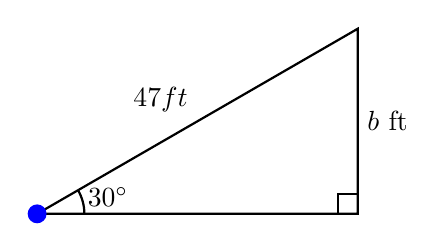
\begin{tikzpicture}[scale=0.1, >=stealth]
  % Coordinates for 30-60-90 triangle
  % Base = 47 * cos(30) = 40.703 ft
  % Height = 47 * sin(30) = 23.5 ft
  \coordinate (A) at (0, 0);          
  % Lower left (30 deg angle)
  \coordinate (B) at (40.703, 0);      
  % Lower right (Right angle)
  \coordinate (C) at (40.703, 23.5);   
  % Top vertex (60 deg angle)
  % Draw Triangle sides
  \draw[thick] (A) -- (B) -- (C) -- cycle;
  % Hypotenuse label
  \path (A) -- (C) node[midway, above left] {$47\text{ ft}$};
  % Height label
  \path (B) -- (C) node[midway, right] {$b$ ft};
  % Right angle mark at B (lower right)
  \draw[thick] (38.203, 0) -- (38.203, 2.5) -- (40.703, 2.5);
  % 30-degree angle arc and label at A (lower left)
  \draw[thick] (6, 0) arc (0:30:6);
  \node at (9, 2.2) {$30^\circ$};
  % Blue circle at lower left vertex
  \fill[blue] (A) circle (1.2);
\end{tikzpicture}
\end{center}

The height, $b$ feet, is the length of the side opposite to 30$^\circ$, so using the definition of the trig ratios (SOH-CAH-TOA) we get the equation
$$\sin(30^\circ) = \frac{\text{opposite to 30}^\circ}{\text{hypotenuse}} = \frac{b}{47}$$
Multiplying each side of the equation by 47 we get 
$$47\sin(30^\circ) = \frac{b}{47} \times 47 = b$$
Rewriting the equation with the variable on the left we have
$$b = 47\sin(30^\circ) = 23.5 \text{ feet}$$
Recall that $b$ measures the height above the center, which is 53 feet, and the gondola sits 3 feet below the wheel. That means Taini will be
$$23.5 + 53 - 3 = 73.5 \text{ feet}$$
high at 30$^\circ$.  

By the way, were you surprised that $47\sin(30^\circ) = 23.5$, such a nice number?  The reason is that 30$^\circ$ sits in one of our special triangles, the 30-60-90 triangle, and $\sin(30^\circ) = \frac{1}{2} = .5$ exactly. 

The variables are $$\theta = \text{ angle of Taini's gondola }(^\circ) \sim \text{indep}$$
$$H = \text{ height of Taini's gondola (feet)} \sim \text{dep}$$
Generalizing our calculation for 30$^\circ$ we see that the equation is $$H = 47 \sin(\theta) + 53 - 3$$ which simplifies to $$H = 47 \sin(\theta) + 50$$

For example, at the next stop of 60$^\circ$, her height is $$H = 47 \sin(60^\circ) + 50 =47 \times \boxed{\texttt{sin}}(60)+50= 90.7031\ldots
\approx 90.7 \text{ feet}$$
We also know that at 180$^\circ$ she is at $53-3 = 50$ feet And that at 270$^\circ$ she is back at $6-3=3$ feet where she got on.

Let's make a table of the values we know so far and use a calculator to find the other values.

\begin{center}
\begin{tabular}{c|c|c|c |c|c|c |c|c|c |c}
    $\theta$ & 0$^\circ$ & 30$^\circ$ & 60$^\circ$ & 90$^\circ$ & 120$^\circ$ & 150$^\circ$ & 180$^\circ$ & 210$^\circ$ & 240$^\circ$ & 270$^\circ$\\ \hline
    $H$ & 50 & 73.5 & 90.7 & 97 & 90.7 & 73.5 & 50 & 26.5 & 9.3 & 3 
\end{tabular}
\end{center}

\subsection*{Circle definitions of the trigonometric ratios}

Wait a minute!  How does our equation make sense for angles that are too big to fit into a right triangle?  For example, how are $\sin(90^\circ)$, $\sin(120^\circ)$, $ \sin(150^\circ)$, $\sin(180^\circ)$, \ldots  defined?  These angles don't fit in a right triangle!

When Taini gets home, she searches the Internet for information on trigonometric ratios. The website explains that sine, cosine, and tangent are defined for any angle, not just angles that fit into a right triangle ($0^\circ < \theta < 90^\circ$).  The extended definition uses circles centered at the origin, the point $(0,0)$. 

Taini draws a picture of a circle with radius 47 feet, the radius of the Ferris Wheel.  She draws an angle, labeled $\theta$ and the radius from the origin to the corresponding point $(x,y)$ on the circle. 

\begin{center}
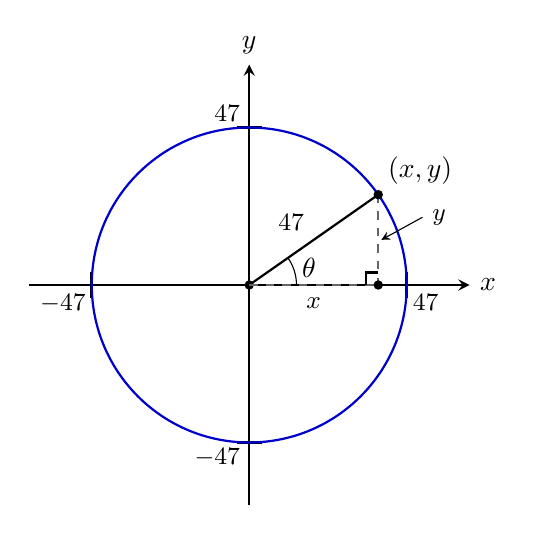
\begin{tikzpicture}[>=stealth, scale=2.0]
  % Grid / Axes
  \draw[->, thick] (-1.4, 0) -- (1.4, 0) node[right] {$x$};
  \draw[->, thick] (0, -1.4) -- (0, 1.4) node[above] {$y$};

  % Tick marks and axis labels at 47 and -47
  \draw[very thick] (1, 0.08) -- (1, -0.08);
  \node[below right, font=\small, inner sep=2pt] at (1, -0.02) {$47$};

  \draw[very thick] (-1, 0.08) -- (-1, -0.08);
  \node[below left, font=\small, inner sep=2pt] at (-1, -0.02) {$-47$};

  \draw[very thick] (0.08, 1) -- (-0.08, 1);
  \node[above left, font=\small, inner sep=2pt] at (-0.02, 1) {$47$};

  \draw[very thick] (0.08, -1) -- (-0.08, -1);
  \node[below left, font=\small, inner sep=2pt] at (-0.02, -1) {$-47$};

  % Circle (rendered at radius 1, labeled as 47)
  \draw[thick, blue!80!black] (0,0) circle (1);

  % Origin
  \fill (0,0) circle (0.03);

  % 35-degree Radius, Right Triangle, and Labels
  \coordinate (O) at (0,0);
  \coordinate (P) at ({cos(35)}, {sin(35)});
  \coordinate (Px) at ({cos(35)}, 0);

  % Right Triangle
  \draw[thick] (O) -- (P);                         % Hypotenuse (Radius)
  \draw[dashed, thick, gray!80!black] (P) -- (Px); % Vertical height
  \draw[dashed, thick, gray!80!black] (O) -- (Px); % Base along x-axis

  % Right angle mark at (Px)
  \draw[thick] ({cos(35) - 0.08}, 0) -- ({cos(35) - 0.08}, 0.08) -- ({cos(35)}, 0.08);

  % Vertex points
  \fill (Px) circle (0.03);
  \fill (P) circle (0.03) node[above right] {$(x,y)$};

  % Angle Arc and Label \theta
  \draw[thin] (0.3, 0) arc (0:35:0.3);
  \node at (0.38, 0.11) {$\theta$};

  % Triangle Side Labels
  \node[above left, font=\small] at ({0.5*cos(35)}, {0.5*sin(35)}) {$47$};
  \node[below, font=\small] at ({0.5*cos(35)}, -0.02) {$x$};
  \draw[<-, thin] ({cos(35) + 0.02}, {0.5*sin(35)}) -- (1.1, {0.75*sin(35)}) node[right, font=\small] {$y$};
\end{tikzpicture}
\end{center}

What does this picture have to do with triangles?  Taini cleverly draws a vertical line from the point on the unit circle to the $x$-axis to get a right triangle. The length of the horizontal leg along the $x$-axis equals the $x$-coordinate of the point on the circle, and the length of the vertical leg equals the $y$-coordinate of the point on the circle. Because the circle has radius 47, the hypotenuse of that triangle is 47.

Taini uses the right triangle definition of sine (SOH-CAH-TOA) to get $$\sin(\theta) = \frac{y}{47} \text{ and } \cos(\theta) = \frac{x}{47}$$

Aha!  These equations can be used to define the sine and cosine for any angle.  That is, for any angle $\theta$, find the point $(x,y)$ on a circle of radius $r$.  Then
$$\sin(\theta) = \frac{y}{r} \text{ and } \cos(\theta) = \frac{x}{r}$$

We can also use these equations to find the $x$- and $y$-coordinates of the point on the circle if we know the radius $r$ and angle $\theta$:
$$x = r\cos(\theta) \text{ and } y = r\sin(\theta)$$

For practice, Taini draws a circle of radius 10 cm on her paper and adds in a line at 130$^\circ$.  

\begin{center}
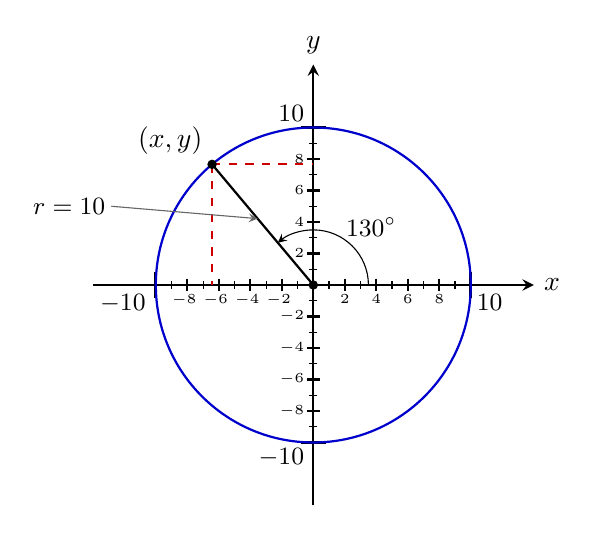
\begin{tikzpicture}[>=stealth, scale=2.0]
  % Grid / Axes
  \draw[->, thick] (-1.4, 0) -- (1.4, 0) node[right] {$x$};
  \draw[->, thick] (0, -1.4) -- (0, 1.4) node[above] {$y$};

  % Unlabeled Intermediate Ticks (1, 3, 5, 7, 9)
  \foreach \pos in {0.1, 0.3, 0.5, 0.7, 0.9} {
    % x-axis
    \draw[thin] (\pos, 0.025) -- (\pos, -0.025);
    \draw[thin] (-\pos, 0.025) -- (-\pos, -0.025);

    % y-axis
    \draw[thin] (0.025, \pos) -- (-0.025, \pos);
    \draw[thin] (0.025, -\pos) -- (-0.025, -\pos);
  }

  % Labeled Tick Marks (2, 4, 6, 8)
  \foreach \val/\pos in {2/0.2, 4/0.4, 6/0.6, 8/0.8} {
    % Positive x-axis
    \draw[thick] (\pos, 0.04) -- (\pos, -0.04);
    \node[below, font=\tiny, inner sep=2pt] at (\pos, -0.02) {$\val$};

    % Negative x-axis
    \draw[thick] (-\pos, 0.04) -- (-\pos, -0.04);
    \node[below, font=\tiny, inner sep=2pt, xshift=-1.2pt] at (-\pos, -0.02) {$-\val$};

    % Positive y-axis
    \draw[thick] (0.04, \pos) -- (-0.04, \pos);
    \node[left, font=\tiny, inner sep=2pt] at (-0.02, \pos) {$\val$};

    % Negative y-axis
    \draw[thick] (0.04, -\pos) -- (-0.04, -\pos);
    \node[left, font=\tiny, inner sep=2pt] at (-0.02, -\pos) {$-\val$};
  }

  % Boundary ticks and labels representing 10 and -10
  \draw[very thick] (1, 0.08) -- (1, -0.08);
  \node[below right, font=\small, inner sep=2pt] at (1, -0.02) {$10$};

  \draw[very thick] (-1, 0.08) -- (-1, -0.08);
  \node[below left, font=\small, inner sep=2pt, xshift=-1.5pt] at (-1, -0.02) {$-10$};

  \draw[very thick] (0.08, 1) -- (-0.08, 1);
  \node[above left, font=\small, inner sep=2pt] at (-0.02, 1) {$10$};

  \draw[very thick] (0.08, -1) -- (-0.08, -1);
  \node[below left, font=\small, inner sep=2pt] at (-0.02, -1) {$-10$};

  % Unit Circle (canvas radius = 1, representing radius 10)
  \draw[thick, blue!80!black] (0,0) circle (1);

  % Origin
  \fill (0,0) circle (0.03);

  % 130-degree Radius and Endpoint
  \coordinate (O) at (0,0);
  \coordinate (P) at ({cos(130)}, {sin(130)});
  \coordinate (Px) at ({cos(130)}, 0);
  \coordinate (Py) at (0, {sin(130)});

  % Red dashed projection lines to axes
  \draw[dashed, thick, red!80!black] (P) -- (Px); % Vertical to x-axis
  \draw[dashed, thick, red!80!black] (P) -- (Py); % Horizontal to y-axis

  % Hypotenuse / Radius Line
  \draw[thick] (O) -- (P);

  % Point P at (x,y)
  \fill (P) circle (0.03) node[above left] {$(x,y)$};

  % Angle Arc with Arrowhead and Label 130°
  \draw[thin, ->] (0.35, 0) arc (0:130:0.35);
  \node at ({0.52*cos(45)}, {0.52*sin(45)}) {\small $130^\circ$};

  % Radius Label 'r=10' positioned at (-1.55, 0.5) with pointer
  \node[font=\small, inner sep=2pt] (rlabel) at (-1.55, 0.5) {$r=10$};
  \draw[thin, ->, gray!80!black] (rlabel.east) -- ({0.55*cos(130)}, {0.55*sin(130)});
\end{tikzpicture}
\end{center}

At the point $(x,y)$ where the line meets the circle, 
it looks like $x \approx -6.5\text{ cm}$ and $y \approx 7.5 \text{ cm}$.  Since the radius is $r = 10 \text{ cm}$, Taini estimates that
$$\sin(130^\circ) \approx \frac{y}{r} = \frac{7.5}{10}=.75$$
and 
$$\cos(130^\circ) \approx \frac{x}{r} = \frac{-6.5}{10}=-.65$$

When she checks on her calculator, she gets
$$\boxed{\texttt{sin}}(130)= 0.7660444431 \approx .77$$
and 
$$\boxed{\texttt{cos}}(130)= -0.6427876097 \approx -.64$$
so her guesses were pretty close.

 \input{GoDoWS}

\noindent \textbf{Do you know \ldots}

\begin{itemize}
\item Why we can't use SOH-CAH-TOA to define the trig ratios of angles larger than 90$^\circ$?
\item How sine and cosine of any angle are defined using a circle?
\item When to use sine or cosine in an applied problem?
\item How to estimate the sine and cosine of an angle using a circle?
\item How to evaluate sine and cosine of angles that end on the $x$-axis or $y$-axis?
 
 \input{NotSure} 
\end{itemize}

\subsection*{Exercises}

\begin{enumerate} 
\item % workbook
Khoeli is working out on a stationary bike.  To warm up, they decide to pedal backward, which causes the pedal to rotate counterclockwise in a circle with a radius of 6.7 inches around a central spindle 11.8 inches above the floor. Let's measure the angle starting at the horizontal line from the center spindle to the front of the bike.
\begin{enumerate}
    \item What is the total height (above the floor) of the pedal when Khoeli's foot is directly forward, level with the spindle?  This is an angle of $0^\circ$.
    \item Repeat for $90^\circ$ when their foot is straight above the spindle and $270^\circ$ when their foot is directly below the spindle.
    \item Use graph paper to draw a circle with radius 6.7 inches centered at the origin (central spindle) and and a line at $320^\circ$ and use your circle to estimate the $y$-coordinate of the point where the line meets the circle.
    \item Use your answer to part (c) to estimate the height of the pedal above the floor when Khoeli has pedaled $320^\circ$. Don't forget the center is 11.8 inches above the floor.
    \item Name the variables and write an equation that describes the height of the pedal above the floor as a function of the rotation angle. Don't forget the units! Hint: your equation should involve sine.
    \item According to your equation, what's the height of the pedal above the floor when Khoeli has pedaled $320^\circ$?  Does your answer agree with your earlier estimate?  (You can check your answers for $0^\circ$, $90^\circ$, and $270^\circ$ too!)
\end{enumerate}

\item %workbook
In Argentina Tango, one dancer moves in a close circle around the other while the center dancer makes highly stylized leg movements in the center. The move is called La Calesita, meaning the carousel. Suppose the turning dancer moves in a circle with a 20 inch radius around their partner, who stays at the center. We can track how far to the left or right the turning dancer is from their partner as a function of the angle they have turned, measured starting from directly to the right ($0^\circ$) and rotating counterclockwise, as usual.
\begin{enumerate}
    \item How far to the left or right of their partner is the turning dancer when they have turned $0^\circ$ (directly to the right)?
    \item Repeat for $90^\circ$ (directly in front) and $180^\circ$ (directly to the left).
    \item Use graph paper to draw a circle with radius 20 inches centered at the origin (partner) and and a line at $250^\circ$ and use your circle to estimate the $x$-coordinate of the point where the line meets the circle.
    \item Use your answer to part (c) to estimate how far to the left or right of their partner the turning dancer is when they have turned $250^\circ$.  
    \item Name the variables, including units, and write an equation illustrating the dependence.  Hint: your equation should involve cosine. 
    \item According to your equation, how far to the left or right of their partner the turning dancer is when they have turned $250^\circ$? Does your answer agree with your earlier estimate?  (You can check your answers for $0^\circ$, $90^\circ$, and $180^\circ$ too!)
\end{enumerate}

\item % workbook
While waiting in a building's lobby for a friend, Aksel notices the glass revolving door at the entrance. The door consists of four glass panels attached to a central pivot.  Each glass panel is 1 meter wide. ``A real-life unit circle,'' Aksel notes with a chuckle,  ``My trig prof would be so proud.''  A \textbf{unit circle} is a circle of radius 1.

As people use the door, Aksel watches the glass panels rotate.  He notices the panel's edge moves from right to left and back again and it moves from close to far and back again.  Here's a top-view of what Aksel sees at a specific time.  Use the diagram to answer the following questions.

\begin{center}
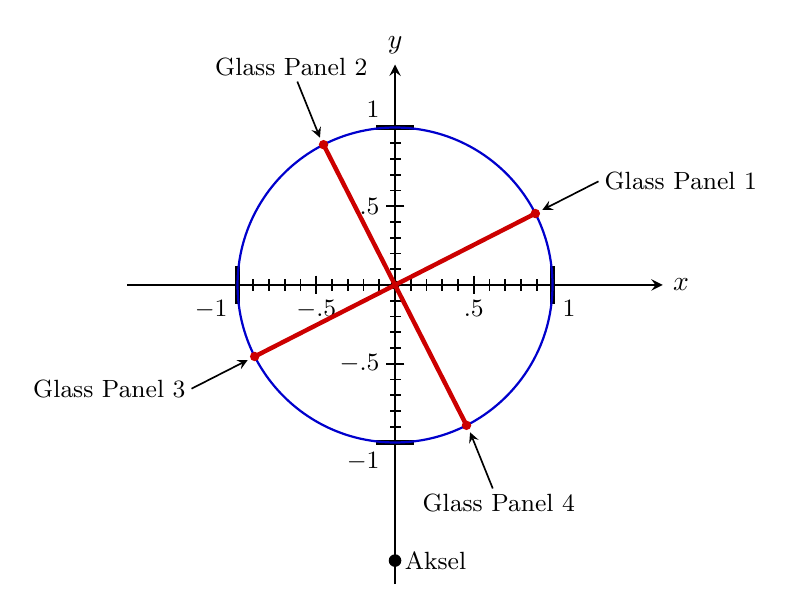
\begin{tikzpicture}[>=stealth, scale=2.0]
  % Grid / Axes
  \draw[->, thick] (-1.7, 0) -- (1.7, 0) node[right] {$x$};
  \draw[->, thick] (0, -1.9) -- (0, 1.4) node[above] {$y$};

  % Small Unlabeled Tick Marks (.1, .2, .3, .4, .6, .7, .8, .9, and negative equivalents)
  \foreach \x in {-0.9, -0.8, -0.7, -0.6, -0.4, -0.3, -0.2, -0.1, 0.1, 0.2, 0.3, 0.4, 0.6, 0.7, 0.8, 0.9} {
    \draw[semithick] (\x, 0.035) -- (\x, -0.035);
    \draw[semithick] (0.035, \x) -- (-0.035, \x);
  }

  % Medium Tick Marks and Labels at 0.5 and -0.5
  \draw[thick] (0.5, 0.06) -- (0.5, -0.06);
  \node[below, font=\small, inner sep=2pt] at (0.5, -0.06) {$.5$};

  \draw[thick] (-0.5, 0.06) -- (-0.5, -0.06);
  \node[below, font=\small, inner sep=2pt] at (-0.5, -0.06) {$-.5$};

  \draw[thick] (0.06, 0.5) -- (-0.06, 0.5);
  \node[left, font=\small, inner sep=2pt] at (-0.06, 0.5) {$.5$};

  \draw[thick] (0.06, -0.5) -- (-0.06, -0.5);
  \node[left, font=\small, inner sep=2pt] at (-0.06, -0.5) {$-.5$};

  % Major Tick Marks and Labels at 1 and -1
  \draw[ultra thick] (1, 0.12) -- (1, -0.12);
  \node[below right, font=\small, inner sep=2pt] at (1.025, -0.06) {$1$};

  \draw[ultra thick] (-1, 0.12) -- (-1, -0.12);
  \node[below left, font=\small, inner sep=2pt] at (-1.025, -0.06) {$-1$};

  \draw[ultra thick] (0.12, 1) -- (-0.12, 1);
  \node[above left, font=\small, inner sep=2pt] at (-0.06, 1.025) {$1$};

  \draw[ultra thick] (0.12, -1) -- (-0.12, -1);
  \node[below left, font=\small, inner sep=2pt] at (-0.06, -1.025) {$-1$};

  % Circle at radius 1
  \draw[thick, blue!80!black] (0,0) circle (1);

  % Origin
  \fill (0,0) circle (0.03);

  % Four Glass Panels (Thick Red Spokes) rotated by 27 degrees
  \draw[ultra thick, red!80!black] (0,0) -- (27:1);
  \draw[ultra thick, red!80!black] (0,0) -- (117:1);
  \draw[ultra thick, red!80!black] (0,0) -- (207:1);
  \draw[ultra thick, red!80!black] (0,0) -- (297:1);

  % Points where the red lines meet the circle
  \fill[red!80!black] (27:1) circle (0.03);
  \fill[red!80!black] (117:1) circle (0.03);
  \fill[red!80!black] (207:1) circle (0.03);
  \fill[red!80!black] (297:1) circle (0.03);

  % Glass Panel Labels and Radial Arrows aligned to panel directions
  % Glass Panel 1 (27°): Text starts ("Glass...") just right of arrow origin at (27:1.45)
  \node[anchor=west, font=\small, inner sep=2pt] at (27:1.45) {Glass Panel 1};
  \draw[->, semithick] (27:1.45) -- (27:1.05);

  % Glass Panel 2 (117°): Center aligned above arrow top
  \node[anchor=south, font=\small, inner sep=2pt] (gp2) at (117:1.45) {Glass Panel 2};
  \draw[->, semithick] (gp2) -- (117:1.05);

  % Glass Panel 3 (207°): Text ends ("...3") just left of arrow origin at (207:1.45)
  \node[anchor=east, font=\small, inner sep=2pt] at (207:1.45) {Glass Panel 3};
  \draw[->, semithick] (207:1.45) -- (207:1.05);

  % Glass Panel 4 (297°): Center aligned below arrow base
  \node[anchor=north, font=\small, inner sep=2pt] (gp4) at (297:1.45) {Glass Panel 4};
  \draw[->, semithick] (gp4) -- (297:1.05);

  % Point at (0, -1.6) labeled Aksel
  \fill (0,-1.75) circle (0.04) node[right, font=\small] {Aksel};

\end{tikzpicture}
\end{center}

\begin{enumerate}
    \item Estimate the $x$-coordinates of each of the four points where the glass panels meet the circle.  Don't forget the units. Be sure to include negative values where appropriate.
    \item What do the $x$-coordinates of the points mean in the story?  
    \item Glass Panel 1 makes an angle of 27$^\circ$ with the positive $x$-axis.  Use that information to determine the angle for Glass Panels 2, 3, and 4.
    \item Write an equation describing how $X$, the $x$-coordinate of the point on the unit circle (in meters), depends on the angle $\phi$ (in degrees).  By the way $\phi$ is the Greek letter phi and is pronounced ``fee''. Hint: the radius of the circle is 1 meter.
    \item Use your equation to check your earlier estimates.
\end{enumerate}

\item %workbook #4
Here's a top-view of what Aksel sees at the moment the four glass panels are vertical and horizontal.

\begin{center}
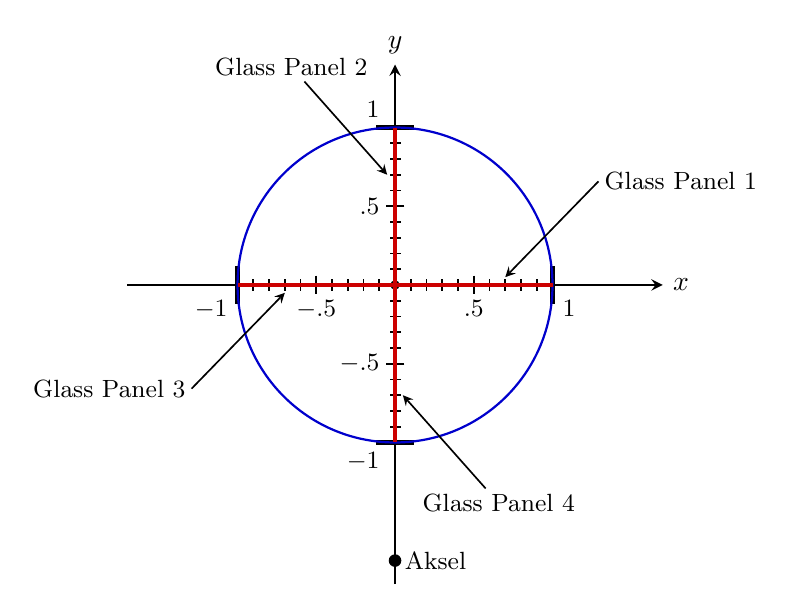
\begin{tikzpicture}[>=stealth, scale=2.0]
  % Grid / Axes
  \draw[->, thick] (-1.7, 0) -- (1.7, 0) node[right] {$x$};
  \draw[->, thick] (0, -1.9) -- (0, 1.4) node[above] {$y$};

  % Small Unlabeled Tick Marks (.1, .2, .3, .4, .6, .7, .8, .9, and negative equivalents) - Slightly longer and thicker
  \foreach \x in {-0.9, -0.8, -0.7, -0.6, -0.4, -0.3, -0.2, -0.1, 0.1, 0.2, 0.3, 0.4, 0.6, 0.7, 0.8, 0.9} {
    \draw[semithick] (\x, 0.035) -- (\x, -0.035);
    \draw[semithick] (0.035, \x) -- (-0.035, \x);
  }

  % Medium Tick Marks and Labels at 0.5 and -0.5
  \draw[thick] (0.5, 0.06) -- (0.5, -0.06);
  \node[below, font=\small, inner sep=2pt] at (0.5, -0.06) {$.5$};

  \draw[thick] (-0.5, 0.06) -- (-0.5, -0.06);
  \node[below, font=\small, inner sep=2pt] at (-0.5, -0.06) {$-.5$};

  \draw[thick] (0.06, 0.5) -- (-0.06, 0.5);
  \node[left, font=\small, inner sep=2pt] at (-0.06, 0.5) {$.5$};

  \draw[thick] (0.06, -0.5) -- (-0.06, -0.5);
  \node[left, font=\small, inner sep=2pt] at (-0.06, -0.5) {$-.5$};

  % Major Tick Marks and Labels at 1 and -1
  \draw[ultra thick] (1, 0.12) -- (1, -0.12);
  \node[below right, font=\small, inner sep=2pt] at (1.025, -0.06) {$1$};

  \draw[ultra thick] (-1, 0.12) -- (-1, -0.12);
  \node[below left, font=\small, inner sep=2pt] at (-1.025, -0.06) {$-1$};

  \draw[ultra thick] (0.12, 1) -- (-0.12, 1);
  \node[above left, font=\small, inner sep=2pt] at (-0.06, 1.025) {$1$};

  \draw[ultra thick] (0.12, -1) -- (-0.12, -1);
  \node[below left, font=\small, inner sep=2pt] at (-0.06, -1.025) {$-1$};

  % Circle at radius 1
  \draw[thick, blue!80!black] (0,0) circle (1);

  % Origin
  \fill (0,0) circle (0.03);

  % Four Glass Panels aligned directly along the axes
  \draw[ultra thick, red!80!black] (0,0) -- (1,0);
  \draw[ultra thick, red!80!black] (0,0) -- (0,1);
  \draw[ultra thick, red!80!black] (0,0) -- (-1,0);
  \draw[ultra thick, red!80!black] (0,0) -- (0,-1);

  % Glass Panel Labels with arrows targeting near the 0.7 mark (shifted 0.05 units off axis)
  % Glass Panel 1: Target (0.7, 0.05)
  \node[anchor=west, font=\small, inner sep=2pt] at (27:1.45) {Glass Panel 1};
  \draw[->, semithick] (27:1.45) -- (0.7, 0.05);

  % Glass Panel 2: Target (-0.05, 0.7)
  \node[anchor=south, font=\small, inner sep=2pt] (gp2) at (117:1.45) {Glass Panel 2};
  \draw[->, semithick] (gp2) -- (-0.05, 0.7);

  % Glass Panel 3: Target (-0.7, -0.05)
  \node[anchor=east, font=\small, inner sep=2pt] at (207:1.45) {Glass Panel 3};
  \draw[->, semithick] (207:1.45) -- (-0.7, -0.05);

  % Glass Panel 4: Target (0.05, -0.7)
  \node[anchor=north, font=\small, inner sep=2pt] (gp4) at (297:1.45) {Glass Panel 4};
  \draw[->, semithick] (gp4) -- (0.05, -0.7);

  % Point at (0, -1.6) labeled Aksel
  \fill (0,-1.75) circle (0.04) node[right, font=\small] {Aksel};

\end{tikzpicture}
\end{center}

\begin{enumerate}
    \item Label each of the four points where the glass panels meet the circle.
    \item Use the $x$-coordinates of those points to evaluate $\cos(0^\circ)$, $\cos(90^\circ)$, $\cos(180^\circ)$, and $\cos(270^\circ)$.
    \item Use the $y$-coordinates of those points to evaluate $\sin(0^\circ)$, $\sin(90^\circ)$, $\sin(180^\circ)$, and $\sin(270^\circ)$.
    \item Check your answers using a calculator.
\end{enumerate}

\item Wind turbines generate electricity as their blades rotate in the wind. A standard wind turbine has a hub located 80 meters above the ground and three blades, each 40 meters long. As a blade rotates, the height of its tip above the ground changes depending on its angle of rotation $\theta$, measured counterclockwise from the positive horizontal position (pointing directly to the right, parallel to the ground).
\begin{enumerate}
    \item What is the height (above ground) of the tip of a blade when the angle has rotated 0$^\circ$?
    \item What is the height (above ground) of the tip of a blade when the angle has rotated 90$^\circ$?
    \item Draw a picture of the wind turbine blade at an angle of 45$^\circ$ and the circle representing the path the tip of the blade travels.  Label the heights and lengths given in the story. Include a vertical line from the tip of the blade to the horizontal line through the hub of the turbine to your picture.  You should have a right triangle with a 45$^\circ$ angle.
    \item What is the height above ground of the tip of the blade when it has rotated 45$^\circ$? Hint: use sine.
    \item Write an equation illustrating how the height of the tip of the blade, $H$ meters above ground, depends on $\theta$, the angle of rotation from the positive horizontal axis.
    \item Make a table. Include the following angles: 0$^\circ$, 45$^\circ$, 90$^\circ$, 135$^\circ$, 180$^\circ$, 225$^\circ$, 270$^\circ$, 315$^\circ$.
\end{enumerate}  %% Gemini

\item Remember Aksel and the revolving door?  Here's an overview picture of a position of the doors at another time.

\begin{center}
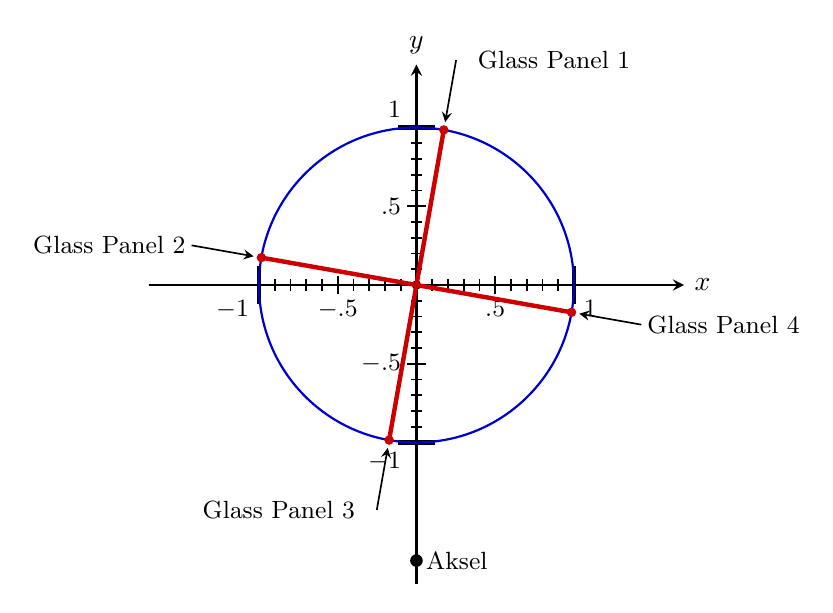
\begin{tikzpicture}[>=stealth, scale=2.0]
  % Grid / Axes
  \draw[->, thick] (-1.7, 0) -- (1.7, 0) node[right] {$x$};
  \draw[->, thick] (0, -1.9) -- (0, 1.4) node[above] {$y$};

  % Small Unlabeled Tick Marks (.1, .2, .3, .4, .6, .7, .8, .9, and negative equivalents)
  \foreach \x in {-0.9, -0.8, -0.7, -0.6, -0.4, -0.3, -0.2, -0.1, 0.1, 0.2, 0.3, 0.4, 0.6, 0.7, 0.8, 0.9} {
    \draw[semithick] (\x, 0.035) -- (\x, -0.035);
    \draw[semithick] (0.035, \x) -- (-0.035, \x);
  }

  % Medium Tick Marks and Labels at 0.5 and -0.5
  \draw[thick] (0.5, 0.06) -- (0.5, -0.06);
  \node[below, font=\small, inner sep=2pt] at (0.5, -0.06) {$.5$};

  \draw[thick] (-0.5, 0.06) -- (-0.5, -0.06);
  \node[below, font=\small, inner sep=2pt] at (-0.5, -0.06) {$-.5$};

  \draw[thick] (0.06, 0.5) -- (-0.06, 0.5);
  \node[left, font=\small, inner sep=2pt] at (-0.06, 0.5) {$.5$};

  \draw[thick] (0.06, -0.5) -- (-0.06, -0.5);
  \node[left, font=\small, inner sep=2pt] at (-0.06, -0.5) {$-.5$};

  % Major Tick Marks and Labels at 1 and -1
  \draw[ultra thick] (1, 0.12) -- (1, -0.12);
  \node[below right, font=\small, inner sep=2pt] at (1.025, -0.06) {$1$};

  \draw[ultra thick] (-1, 0.12) -- (-1, -0.12);
  \node[below left, font=\small, inner sep=2pt] at (-1.025, -0.06) {$-1$};

  \draw[ultra thick] (0.12, 1) -- (-0.12, 1);
  \node[above left, font=\small, inner sep=2pt] at (-0.06, 1.025) {$1$};

  \draw[ultra thick] (0.12, -1) -- (-0.12, -1);
  \node[below left, font=\small, inner sep=2pt] at (-0.06, -1.025) {$-1$};

  % Circle at radius 1
  \draw[thick, blue!80!black] (0,0) circle (1);

  % Origin
  \fill (0,0) circle (0.03);

  % Four Glass Panels (Thick Red Spokes) rotated by 80 degrees
  \draw[ultra thick, red!80!black] (0,0) -- (80:1);
  \draw[ultra thick, red!80!black] (0,0) -- (170:1);
  \draw[ultra thick, red!80!black] (0,0) -- (260:1);
  \draw[ultra thick, red!80!black] (0,0) -- (350:1);

  % Points where the red lines meet the circle
  \fill[red!80!black] (80:1) circle (0.03);
  \fill[red!80!black] (170:1) circle (0.03);
  \fill[red!80!black] (260:1) circle (0.03);
  \fill[red!80!black] (350:1) circle (0.03);

  % Glass Panel Labels and Radial Arrows
  % Glass Panel 1 (80°): Label shifted right (anchor=west) while arrow remains pointing to (80:1.05)
  \node[anchor=west, font=\small, inner sep=2pt] at ({1.45*cos(80) + 0.1}, {1.45*sin(80)}) {Glass Panel 1};
  \draw[->, semithick] (80:1.45) -- (80:1.05);

  % Glass Panel 2 (170°): Text ends just left of arrow origin
  \node[anchor=east, font=\small, inner sep=2pt] at (170:1.45) {Glass Panel 2};
  \draw[->, semithick] (170:1.45) -- (170:1.05);

  % Glass Panel 3 (260°): Label shifted left (anchor=east) while arrow remains pointing to (260:1.05)
  \node[anchor=east, font=\small, inner sep=2pt] at ({1.45*cos(260) - 0.1}, {1.45*sin(260)}) {Glass Panel 3};
  \draw[->, semithick] (260:1.45) -- (260:1.05);

  % Glass Panel 4 (350°): Text starts just right of arrow origin
  \node[anchor=west, font=\small, inner sep=2pt] at (350:1.45) {Glass Panel 4};
  \draw[->, semithick] (350:1.45) -- (350:1.05);

  % Point at (0, -1.75) labeled Aksel
  \fill (0,-1.75) circle (0.04) node[right, font=\small] {Aksel};

\end{tikzpicture}
\end{center}
\begin{enumerate}
    \item Estimate the $y$-coordinates of each of the four points where the glass panels meet the circle.  Don't forget the units. Be sure to include negative values where appropriate.
    \item What do the $y$-coordinates of the points mean in the story?  
    \item Glass Panel 1 makes an angle of 80$^\circ$ with the positive $x$-axis.  Use that information to determine the angle for Glass Panels 2, 3, and 4.
    \item Write an equation describing how $Y$, the $y$-coordinate of the point on the unit circle (in meters), depends on the angle $\phi$ (in degrees).  Hint: the radius of the circle is 1 meter.
    \item Use your equation to check your earlier estimates.
\end{enumerate}

\item Miakoda works at an industrial warehouse that uses a security sensor mounted on a fixed post in the center of the room. The sensor beam extends 10 meters and continuously rotates in a full circle around the post to scan for obstacles.  As the beam rotates, the angle $\beta$ is measured counterclockwise from due East ($0^\circ$). There is a storage rack along a line 5 meters East of the center post that holds valuable equipment. Miakoda is interested in determining the angles where the sensor beam reaches the storage rack line.
\begin{enumerate}
    \item She wonders if the sensor beam reach the storage rack line at an angle of 50$^\circ$.  Will it?  Repeat for $-50^\circ$.  What do you notice.
    \item Will the sensor beam reach the storage rack line at an angle of 70$^\circ$?  Repeat for $-70^\circ$.  What do you notice.
    \item Let's write $D$ for the distance the sensor beam reaches horizontally (in meters). Write an equation describing how $D$ is a function of the angle $\beta$.
    \item At what angles (one positive and one negative) does the beam reach exactly 5 meters where the storage rack is?  Hint: use arccos.
\end{enumerate}

\end{enumerate}

\bigskip

\noindent \textbf{When you're done \ldots}

\begin{itemize}
\item Don't forget to check your answers with those in the back of the textbook. 
\item Not sure if your answers are close enough? Compare with a classmate or ask the instructor.  
\item Getting the wrong answers or stuck on a problem?  Re-read the section and try the problem again. If you're still stuck, work with a classmate or go to your instructor's office hours.
\item It's normal to find some parts of some problems difficult, but if all the problems are giving you grief, be sure to talk with your instructor or advisor about it.  They might be able to suggest strategies or support services that can help you succeed.
\item Make a list of key ideas or processes to remember from the section.  The ``Do you know?'' questions can be a good starting point.
\end{itemize}


